\begin{figure}
\centering
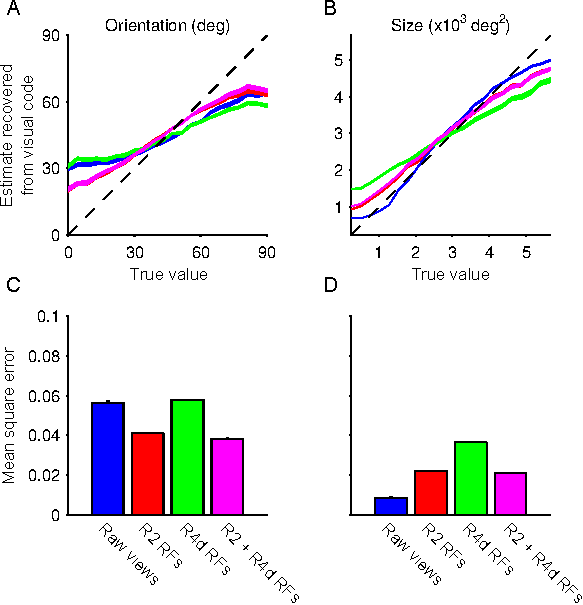
\includegraphics{figures/orsi}
\caption{Analysing the shape information encoded by R2 cells.
Neural networks can be trained to estimate the orientation, size and elevation of visual stimuli simultaneously ($N=1000$).
Details of the figure are the same as for Figure~\ref{fig:elaz}.
A: Network performance for stimulus orientation.
Orientation was constrained between 0\degree\ and 90\degree\ to avoid the problem of aliasing.
B: Network performance for stimulus size.
This parameter is easy for networks to calculate as a linear combination of inputs.
C: Network performance for stimulus elevation.
Performance is poorer at the extremes of values where the stimuli are only partially within the visual field.
D--F: Mean square error for each combination of parameter varied and network type.
As with the elevation + azimuth networks (Figure~\ref{fig:elaz}), performance was best with raw views but adequate with the sets of ring neuron inputs.
}
\label{fig:orsi}
\end{figure}
